\documentclass[11pt]{article}
\usepackage[a4paper,margin=2.5cm]{geometry}
\usepackage{amsmath,amssymb}
\usepackage{graphicx}
\usepackage{booktabs}
\usepackage{hyperref}

% 验收文档（英文正文 + 中文注释）：
% 1. 多个 section、公式、图表、参考文献与 \input 子文件，覆盖常见编译需求；
% 2. 保留几处可改的句子，便于测试「agent 改动 → 变更审阅 → 接受/放弃」。

\title{A Minimal Document for the DSH LaTeX Workbench}
\author{Local test}
\date{\today}

\begin{document}
\maketitle

\section{Introduction}
This is the first paragraph of the acceptance document. It is long enough to wrap
over several lines, which gives SyncTeX a stable line-level mapping. Clicking
anywhere in the PDF should resolve back to one of the lines below — try it: point
at this sentence and write a note.

% [AI suggestion] 按批注压缩：原三行并成一句，保留「保存即刷新、无需手动 pdflatex」的结论。
Live compilation keeps the sidebar PDF current: saving a \texttt{.tex} file triggers
a rebuild, with no manual \texttt{pdflatex} run.

\section{An equation}
The action of a scalar field in flat spacetime is
\begin{equation}
  S[\phi] = \int d^4x \left( \frac{1}{2}\partial_\mu\phi\,\partial^\mu\phi
    - \frac{1}{2}m^2\phi^2 - \frac{\lambda}{4!}\phi^4 \right),
  \label{eq:action}
\end{equation}
and its equation of motion reads
\begin{equation}
  \left(\Box + m^2\right)\phi + \frac{\lambda}{3!}\phi^3 = 0 .
  \label{eq:eom}
\end{equation}
Equations~\eqref{eq:action} and~\eqref{eq:eom} exercise the coordinate mapping
inside display math.

\section{A figure}
Figure~\ref{fig:phase} is included from \texttt{figures/phase.pdf}, which checks
that relative graphics paths resolve when the build directory lives elsewhere.
\begin{figure}[htbp]
  \centering
  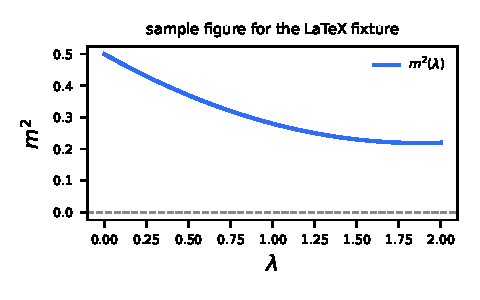
\includegraphics[width=0.62\linewidth]{figures/phase.pdf}
  \caption{A vector figure included from a subdirectory.}
  \label{fig:phase}
\end{figure}

\section{A table}
Table~\ref{tab:checks} uses \texttt{booktabs} rules and a \texttt{tabular}.
\begin{table}[htbp]
  \centering
  \begin{tabular}{lll}
    \toprule
    Check & Command & Expected \\
    \midrule
    compile & \texttt{latexmk} & one PDF, no manual rerun \\
    locate & \texttt{synctex} & matching source line \\
    review & diff & one hunk per edit \\
    \bottomrule
  \end{tabular}
  \caption{The three checks this fixture is meant to exercise.}
  \label{tab:checks}
\end{table}

\section{Citations}
Citations come from \texttt{refs.bib} through BibTeX:~\cite{sample2024} describes
a placeholder article, while~\cite{sample2023} is a placeholder conference paper.
A missing entry would surface as an undefined-citation warning in the log.

\section{Checklist}
This section lists three checks:
\begin{itemize}
  \item the document compiles and reports a page count;
  \item clicking the PDF jumps to the matching \texttt{.tex} line;
  \item editing one line here produces exactly one reviewable change.
\end{itemize}

% 子文件：验证 \input 与多文件改动审阅（改这一行应只产生一个 hunk）
\section{Appendix: multi-file input}
This paragraph lives in \texttt{sections/appendix.tex} and is pulled in with
\texttt{\textbackslash input}. Editing it should show up as a change in that file,
not in the main document.


\section{Conclusion}
If all three checks pass, compilation, two-way navigation and change review are
all wired up.

\bibliographystyle{plain}
\bibliography{refs}

\end{document}
